% Template for Cogsci submission with R Markdown

% Stuff changed from original Markdown PLOS Template
\documentclass[10pt, letterpaper]{article}

\usepackage{cogsci}
\usepackage{pslatex}
\usepackage{float}
\usepackage{caption}

% amsmath package, useful for mathematical formulas
\usepackage{amsmath}

% amssymb package, useful for mathematical symbols
\usepackage{amssymb}

% hyperref package, useful for hyperlinks
\usepackage{hyperref}

% graphicx package, useful for including eps and pdf graphics
% include graphics with the command \includegraphics
\usepackage{graphicx}

% Sweave(-like)
\usepackage{fancyvrb}
\DefineVerbatimEnvironment{Sinput}{Verbatim}{fontshape=sl}
\DefineVerbatimEnvironment{Soutput}{Verbatim}{}
\DefineVerbatimEnvironment{Scode}{Verbatim}{fontshape=sl}
\newenvironment{Schunk}{}{}
\DefineVerbatimEnvironment{Code}{Verbatim}{}
\DefineVerbatimEnvironment{CodeInput}{Verbatim}{fontshape=sl}
\DefineVerbatimEnvironment{CodeOutput}{Verbatim}{}
\newenvironment{CodeChunk}{}{}

% cite package, to clean up citations in the main text. Do not remove.
\usepackage{cite}

\usepackage{color}

% Use doublespacing - comment out for single spacing
%\usepackage{setspace}
%\doublespacing


% % Text layout
% \topmargin 0.0cm
% \oddsidemargin 0.5cm
% \evensidemargin 0.5cm
% \textwidth 16cm
% \textheight 21cm

\title{An information-seeking account of eye movements during spoken and signed
language comprehension}


\author{ {\large \bf Kyle MacDonald}$^1$ (kylem4@stanford.edu), {\large \bf Aviva Blonder}$^2$ (aviva.blonder@oberlin.edu), \\  {\large \bf Virginia Marchman}$^1$ (marchman@stanford.edu), {\large \bf Anne Fernald}$^1$ (afernald@stanford.edu), \\ {\large \bf Michael C. Frank}$^1$ (mcfrank@stanford.edu)  \AND
   $^1$ Department of Psychology Stanford University, $^2$ Department of Psychology Oberlin University}

\begin{document}

\maketitle

\begin{abstract}
Language comprehension involves intergrating information from the
linguistic signal and the surrounding world. But how do we allocate our
limited cognitive resources to gather different kinds of information? In
the current work, we propose that the language comprehension system
adapts to different tradeoffs between the value of gathering linguistic
information and the value of fixating on the nonlingustic visual world.
We use two case studies of eye movements during language comprehension
to test predictions of our account. First, we show that, compared to
children processing spoken language, young visual language learners (a)
delayed eye movements away from a language source, (b) were more
accurate with their initial shifts, and (c) produced a smaller
proportion of nonlanguage-driven, exploratory gaze shifts (Experiment
1). Next, we present a well-controlled, confirmatory test of our
account, showing that English-speaking adults produced fewer
nonlanguage-driven eye movements when processing displays of printed
text compared to spoken language (Experiment 2). Together, these data
suggest that the language comprehension system responds to changes in
the value of seeking different kinds of information to increase the
chance of rapid and accurate language understanding.

\textbf{Keywords:}
eye movements; language processing; information-seeking; American Sign
Language; drift diffusion models
\end{abstract}

\section{Introduction}\label{introduction}

Language comprehension involves the rapid integration of linguistic
information with information about the surrounding world.\footnote{Here
  we focus on the task of reference resolution where an interlocutor
  produces an utterance that refers to a concrete object in the visual
  scene.} For example, imagine there is only one red object amongst many
others, and you hear someone say, ``Pass me the red \_\_\_\_\_!'' If you
have successfully encoded the visual world, then the adjective ``red''
allows you to constrain the speaker's intended meaning and respond
rapidly and accurately. However, for this integration process to work,
we must monitor multiple streams of information in real-time using a
limited set of cognitive resources. So how do we decide when to gather
information about language and when to gather information about the
world? We propose that the language comprehension system modulates
behavior in response to changes in the value of gathering different
kinds of information. We test our information-seeking account using two
case studies that manipulate the value of eye movements during language
processing: a) a comparison of signed and spoken language processing and
b) a comparison of spoken language processing and the processing of
printed text.

The study of eye movements during language comprehension has provided
insight into the interaction between conceptual representations of the
world and the incoming linguistic signal. For example, work on spoken
language processing shows that adults will rapidly shift visual
attention upon hearing the name of an object in the visual scene, with a
high proportion of these shifts occurring prior to the offset of the
target word (Allopenna, Magnuson, \& Tanenhaus, 1998; Tanenhaus,
Spivey-Knowlton, Eberhard, \& Sedivy, 1995). Moreover, researchers have
found that conceptual representations activated by the visual world can
modulate subsequent eye movements during language processing (Altmann \&
Kamide, 2007). The majority of this work has leveraged eye movements as
an index of the underlying language comprehension process but has
focused less on the top-down influence of participants' goals on
fixation patterns (see Salverda et al., 2011 for a review).

In contrast, researchers in the fields of natural vision and
decision-making have modeled eye movements as a tool for information
gathering (Ballard \& Hayhoe, 2009) and a reflection of the underlying
components of the decision-making process (Shadlen \& Kiani, 2013). In
this approach, the participant's goal becomes critical for understanding
the timing and location of fixations, and the function of eye movements
is to reduce uncertainty about the external world to maximize the
expected reward of future actions. For example, Hayhoe \& Ballard (2005)
review evidence that people do not fixate on the most salient aspects of
the visual scene, but instead focus on aspects that are most helpful for
the current task such as gaze shifts to an upcoming obstacle when
walking.

In the current work, we leverage aspects of the information-seeking
framework to account for a wider variety of fixation patterns during
language comprehension. We characterize eye movements as a tradeoff
between gathering more information about the visual world and gathering
more information about the incoming linguistic signal. We assume that
the goal of the language comprehension system is to generate behaviors
that maximize the probability of making the correct future response (in
the context of our task, resolving reference rapidly and accurately). To
test the predictions of our account, we present two case studies where
multiple kinds of information must be gathered using the same input
mechanism -- vision: a) processing a visual-manual language, e.g.,
American Sign Language (ASL), and b) processing displays of printed
text. Our key prediction is that competition for visual attention would
make eye movements to the visual world less valuable, leading people to
gather more information about the linguistic signal and generate a
higher proportion of language-driven gaze shifts.

\begin{CodeChunk}
\begin{figure}[t]

{\centering 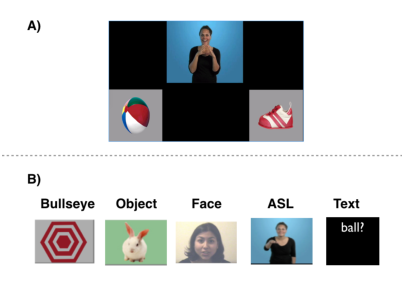
\includegraphics{figs/e1_stimuli-1} 

}

\caption[Stimuli information for Experiments 1 and 2]{Stimuli information for Experiments 1 and 2. Panel A shows the layout of the three potential fixation locations across all the tasks: the center stimulus, the target picture, and the distracter picture. Panel B shows the five different center stimulus items from Experiments 1 and 2: a person signing (ASL), a person speaking (Face), a static image of a familiar object (Object), a static geometric shape (Bullseye), and printed text (Text).}\label{fig:e1_stimuli}
\end{figure}
\end{CodeChunk}

\begin{CodeChunk}
\begin{figure*}[t]

{\centering 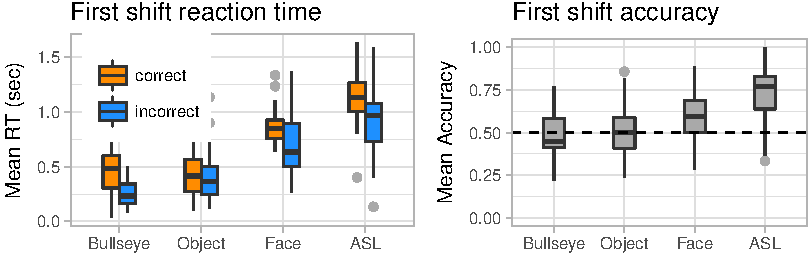
\includegraphics{figs/e1_acc_rt_plot-1} 

}

\caption[First shift accuracy and Reaction times (RT) from Experiment 1]{First shift accuracy and Reaction times (RT) from Experiment 1. The left panel shows a boxplot representing the distribution of RTs for correct (orange) and incorrect (blue) shifts for each center stimulus type. The right panel shows the distribution of mean first shift accuracy scores for each center stimulus type. The solid lines represents median values, the boundaries of the box show the upper and lower quartiles, and the whiskers show the full range of the data excluding outliers.}\label{fig:e1_acc_rt_plot}
\end{figure*}
\end{CodeChunk}

\section{Experiment 1}\label{experiment-1}

Experiment 1 provides an initial test of our information-seeking
account. We directly compared eye movements of children learning a
visual language to children learning a spoken language using two
parallel, 3-alternative forced choice real-time language comprehension
tasks. We predicted that the task of processing a visual language would
increase the value of fixating on the language source and decrease the
value of generating exploratory, nonlanguage-driven shifts to the visual
world. To test this prediction, we use a combination of behavioral and
model-based analyses.

\subsection{Method}\label{method}

\subsubsection{Participants}\label{participants}

\begin{table}[b]
\centering
\begin{tabular}{lrrrr}
  \hline
Task & Mean\_Age & Min\_Age & Max\_Age & n \\ 
  \hline
ASL & 27.60 &  16 &  53 &  27 \\ 
  Face & 26.00 &  25 &  26 &  24 \\ 
  Object & 31.90 &  26 &  39 &  40 \\ 
  Bullseye & 26.10 &  26 &  27 &  16 \\ 
   \hline
\end{tabular}
\caption{Age distributions of child participants in Experiment 1.} 
\end{table}

\emph{ASL sample.} Participants were 27 native, monolingual ASL-learning
children (14 deaf, 13 hearing, M\_Age= 28.5 months, range = 16-53
months). The sample consisted of both deaf children of deaf adults and
hearing children of deaf adults (CODAs). All children, regardless of
hearing status, were exposed to ASL from birth through extensive
interaction with at least one caregiver fluent in ASL and were reported
to experience at least 80\% ASL in their daily lives. We excluded a
small number of participants because they did not complete the task due
to inattentiveness or parental interference (n = 5).

\emph{Spoken English samples.} Participants were 80 native, monolingual
English-learning children divided across three different samples (age
range = 25-39 months). Participants had no reported history of
developmental or language delay. All participants were judged to be
primarily English- language learners, based on parental report on
linguistic input. Several participants were excluded from each of the
task for not completing the task because of inattentiveness (Face: n =
1; Bull: n = 5; Object: n = TODO).

Table 1 contains details about the age distributions of children in all
of four tasks. We would like to note that the ASL sample included a
wider age range compared to the spoken English samples. This is because
native ASL learners are a difficult population to recruit, with the
incidence of deafness at birth in the US being less than .003\%, and
only 10\% of the 2-3 per 1000 children born with hearing loss have a
deaf parent who is likely to be fluent in ASL (Mitchell \& Karchmer,
2004). However, we included age as a covariate in all of our group
comparisons and report any age effects.

\subsubsection{Stimuli}\label{stimuli}

\emph{ASL linguistic stimuli.} We recorded two separate sets of ASL
stimuli. Both sets were recorded with a native ASL signer, using
alternative ASL sentence structures for asking questions: 1)
Sentence-initial wh-phrase: ``HEY! WHERE {[}target noun{]}?'' and 2)
Sentence-final wh-phrase: ``HEY! {[}target noun{]} WHERE?'' To prepare
the stimuli, two female native ASL users recorded several tokens of each
sentence in a child-directed register. Before each sentence, the signer
produced a hand-wave gesture commonly used in ASL to gain an
interlocutor's attention before initiating an utterance. The final
tokens were chosen based on naturalness.

\emph{ASL visual stimuli.} The image set consisted of colorful digitized
pictures of objects presented in fixed pairs, in which the object names
had no phonological overlap (cat---bird, car---book, bear---doll,
ball---shoe). Images were digitized pictures presented in fixed pairs,
matched for visual salience with 3--4 tokens of each object type. Each
object served as target four times and as distracter four times. Side of
target picture was counterbalanced across trials.

\emph{English linguistic stimuli.} All three tasks (Object, Bullseye,
and Face) featured the same female native speaker of English. The
speaker used natural child-directed speech and recorded sentences with
the following structure: ``Look! Where's the (target word)?''\footnote{We
  would like to point out that even though there are significant
  differences between ASL and English question structures, all stimulus
  sets had the same trial structure: language to attract participants'
  attention followed by a sentence containing a target noun.} The target
words consisted of six familiar labels to match the six familiar
objects: ball, banana, book, cookie, juice, and shoe.

\emph{English video stimuli.} For the Face task, we recorded the female
native English speaker as she looked straight ahead and said, ``Look!
Where's the (target word)?'' This video served as both a center stimulus
and the source of the speech information. The video was the same size as
the pictures. One video was prepared for each of the six objects. The
final videos were chosen based on naturalness.

\emph{English visual stimuli.} Features of the image set were similar to
the ASL task. The image set consisted of six objects corresponding to
words judged to be highly familiar to children of this age: ball,
banana, book, cookie, juice, and shoes. 3--4 tokens of each of the six
objects appeared throughout the experiment and side of target picture
was counterbalanced across trials.

\subsubsection{Design and procedure}\label{design-and-procedure}

Participants viewed the ASL task on a 27" monitor. Children sat on their
caregiver's lap, and the child's gaze was recorded using a digital
camcorder set up behind the monitor. On each trial, pictures of two
familiar objects appeared on the screen, a target object corresponding
to the target noun, and a distracter object matched for visual salience.
Between the two pictures was a central video of an adult female signing
the name of one of the pictures. Participants saw 32 test trials with
five filler trials (e.g. ``YOU LIKE PICTURES? MORE WANT?'') interspersed
to maintain children's interest.

Participants viewed the Face, Object, and Bullseye tasks on a large
projector screen in a sound-treated testing booth. Similar to the ASL
task, at the beginning of each test trial, pictures of two familiar
objects appeared on the screen and then a center stimulus appeared
between the two pictures. The center stimulus varied across the three
tasks: Face, Object, and Bullseye (see Figure 1 for details).
Participants saw approximately 32 test trials with several filler trials
interspersed to maintain children's interest.

\emph{Trial structure.} On each trial, the child saw two images of
familiar objects on the screen for two seconds before the center
stimulus (a signer) appeared. This time allowed the child to visually
explore both images. Next, the target sentence -- which consisted of a
carrier phrase, target noun, and question sign -- was presented,
followed by two seconds without language to allow the child to respond
to the signer's sentence. The trial structure of the Face, Object, and
Bullseye tasks were highly similar: children were given two seconds to
visually explore the objects prior to the appearance of the center
stimulus, then processed a target sentence, and finally were given two
seconds of silence to generate a response to the target noun.

\emph{Coding.} Participants' gaze patterns were videotaped and later
coded frame-by-frame at 33-ms resolution by trained coders blind to
target side. On each trial, coders indicated whether the eyes were
fixated on the central signer, one of the images, shifting between
pictures, or away (off), yielding a high-resolution record of eye
movements aligned with target noun onset. Prior to coding, all trials
were pre-screened to exclude those few trials on which the participant
was inattentive or there was external interference.

\subsubsection{Behavioral measures}\label{behavioral-measures}

\emph{Reaction time.} Reaction time (RT) corresponds to the latency to
shift from the central stimulus to either the target or the distracter
pictures measured from target-noun onset. We chose to cutoff RTs longer
than two seconds since these shifts are unlikely to be generated in
response to the incoming language stimulus (see Ratcliff, 1993).

\emph{First shift accuracy.} Accuracy was the mean proportion of first
shifts that landed on the target picture out of the total number of
shifts that landed on either the target or the distracter picture over a
two-second window from target noun onset. This measure reflects the
accuracy of language-driven saccades to the visual world. Mean first
shift accuracy scores were computed for each participant for both
correct and incorrect shifts. Trials where the participants did not
generate a shift were not included in the computation.

\begin{CodeChunk}
\begin{figure}[t]

{\centering 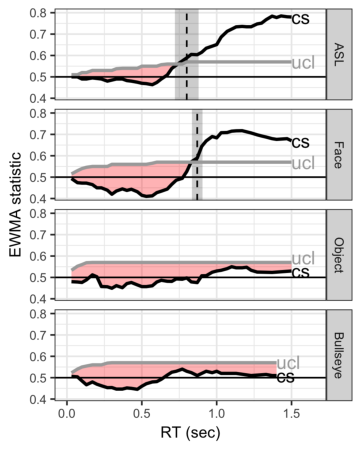
\includegraphics{figs/e1_control_chart-1} 

}

\caption[Output for the EWMA guessing model for all center stimulus types in Experiment 1]{Output for the EWMA guessing model for all center stimulus types in Experiment 1. The black curve represents the evolution of the control statistic (cs) as a function of reaction time. The grey curve represents the upper control limit (ucl). The vertical dashed line is the median cutoff value (point when the control process shifts out of a guessing state) across all participants. The grey shaded area represents the 95\% confidence interval around the estimate of the median cutoff point. And the shaded red area represents the proprotion of responses that were flagged as guesses by the EWMA model.}\label{fig:e1_control_chart}
\end{figure}
\end{CodeChunk}

\begin{CodeChunk}
\begin{figure}[t]

{\centering 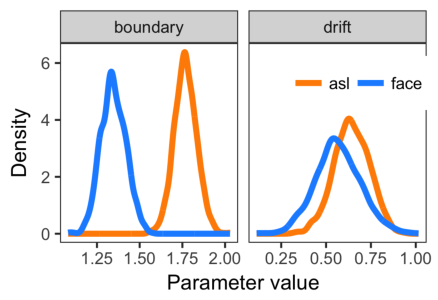
\includegraphics{figs/e1_hddm_plot-1} 

}

\caption[Posterior distributions over the boundary and drift rate parameters in the heirarchical drift diffusion model]{Posterior distributions over the boundary and drift rate parameters in the heirarchical drift diffusion model.}\label{fig:e1_hddm_plot}
\end{figure}
\end{CodeChunk}

\subsection{Results and Discussion}\label{results-and-discussion}

\subsubsection{Analysis plan}\label{analysis-plan}

First, we present behavioral analyses of accuracy and RT. Since RTs are
not normally distributed, we log transformed all RTs for our statistical
analyses. To quantify differences between groups, we used the
\texttt{lme4} R package (Bates, Maechler, Bolker, \& Walker, 2013) to
fit mixed-effects regression models that included a by-subject random
intercept to account for repeated measures from each participant. All
data and analysis code can be found in the online repository for this
project: \url{https://github.com/kemacdonald/speed-acc}.

Next, we present two model-based analyses that quantify different
patterns of eye movements across the four language comprehension tasks.
First, we use an Exponentially weighted moving average (EWMA) method
(Vandekerckhove \& Tuerlinckx, 2007) to model the proportion of
nonlanguage-driven shifts away from the center stimulus to the visual
world. The goal of the EWMA is to identify whether a process has
deviated from a pre-defined ``control state'' by taking into account the
prior behavior of the process, weigting recent obeservations more
heavily The model generates two values: a ``control statistic'' (CS) and
an ``upper control limit'' (UCL) for each point in the RT distribution.
Once the CS becomes larger than the UCL, the process is determined to
have exited the control state.\footnote{\(c_s = \lambda x_s + (1-\lambda)c_{s-1}\)
  where the \(\lambda\) parameter determines the number of prior RTs
  that are included in the moving average computation.
  \(UCL_s = c_0 + L\sigma_0\sqrt{\frac{\lambda}{2-\lambda}[1-(1-\lambda)^{2s}]}\)
  where \(L\) controls the width of the control limits with higher
  values leading to a more conservative test. We chose values used in
  prior work using the EWMA with speeded decision tasks (Vandekerckhove
  \& Tuerlinckx, 2007)}

Here, we adapt the EWMA approach to model changes in the process that
generate eye movements away from the center stimulus to the visual
world. We define the control state as an expectation of
nonlanguage-driven shifts and model this as a Bernoulli process with
probability of success 0.5. As the sentence unfolds, we assume that
participants gather more of the linguistic information prior to shifting
and the underlying process should bias towards more accurate shifts or a
Bernoulli process with probability success \textgreater{} 0.5. With this
model, we can compare across our groups: a) the cutoff point when the CS
exceeded the UCL indicating that participants started to generate
language-driven shifts and b) the proportion of shifts that the model
categorizes as language-driven vs.~exploratory.

Finally, we use Drift diffusion models (DDMs) (Ratcliff \& Childers,
2015) to quantify differences in the dynamics of speed and accuracy for
eye movements generated in response to the incoming linguistic signal.
DDMs form a class of sequential decision-making models designed
specifically for rapid two-alternative forced choice tasks. The model
assumes that people accumulate noisy evidence in favor of one
alternative with a response generated when the evidence crosses a
pre-defined decision threshold. The DDM approach is useful because it
can account for all components of the behavioral response: correct and
incorrect RT distributions. Moreover, the parameters of the DDM map onto
meaningful psychological variables of interest. Here we focus on two of
these parameters: \textbf{boundary separation}, which maps onto the
amount of evidence gathered before generating a response (higher values
suggest a prioritization of accuracy over speed) and \textbf{drift
rate}, which maps onto the amount of evidence that is accumulated per
unit time (higher values indicate more efficient processing).

We chose to implement a hierarchical Bayesian version of the DDM using
the HDDM Python package (Wiecki, Sofer, \& Frank, 2013) because we were
dealing with relatively few trials from child participants and recent
simulation studies have shown that the HDDM approach was better than
other DDM fitting methods when the number of observations was small
(Ratcliff \& Childers, 2015).

\subsubsection{Behavioral analyses}\label{behavioral-analyses}

\emph{RT.} Panel A of Figure 2 shows children's RTs for correct and
incorrect shifts. Visual inspection of the figure suggests that there
was a speed accuracy tradeoff in the ASL, Face, and Bullseye conditions
where incorrect RTs tended to be faster than correct RTs. To quantify
differences across the groups, we fit a linear mixed-effects regression
predicting first shift RT as a function of center stimulus type,
controlling for age, and including user-defined contrasts to test
specific comparisons of interest:
\texttt{Log(RT) $\sim$ center stimulus type + age +  (1 | subject)}. We
found that (a) ASL learners delayed their shifts compared to all of the
spoken English participants (\(\beta\) = -0.96, \(p\) \textless{} .001),
(b) ASL learners' shifts were slower compared to participants in the
Face task (\(\beta\) = -0.42, \(p\) \textless{} .001), and (c)
participants in the Face task shifted slower compared to participants in
the Object and Bullseye tasks (\(\beta\) = -0.73, \(p\) \textless{}
.001).

\emph{Accuracy.} Next we compared the accuracy of first shifts across
the different tasks by fitting a mixed-effects logistic regression with
the same specifications and contrasts as the RT model. We found that (a)
ASL learners were more accurate compared to all of the spoken English
participants (\(\beta\) = -0.69, \(p\) \textless{} .001), (b) ASL
learners were more accurate when directly compared to participants in
the Face task (\(\beta\) = -0.54, \(p\) = 0.001), and (c) participants
in the Face task were numerically more accurate compared to participants
in the Object and Bullseye tasks (\(\beta\) = -0.73) but this effect was
not significant at the .05 level (\(p\) = 0.094).

\subsubsection{Model-based analyses}\label{model-based-analyses}

\emph{EWMA.} Figure 3 shows the output of the EWMA model for the four
different center stimulus types. This plot shows changes in the control
statistic (CS) and the upper control limit (UCL) as a function of
participants' reaction times. Each CS starts at chance performance and
below the UCL. In the ASL and Face tasks, the CS values begin to
increase with RTs around 0.7 seconds after noun onset eventually
exceeding the UCL and entering a nonguessing state. In contrast, the CS
in the Object and Bullseye tasks never crosses the UCL, meaning that
children's first shifts were equally likely to land on the target as on
the distracter, regardless of when those shifts were initiated in the RT
distribution. This result suggests that first shifts in the
Bullseye/Object tasks are language-driven and may instead reflect a
different process such as gathering more information about the referents
in the visual world.

Next, we compared the EWMA output of participants in the ASL and Face
tasks. We found that ASL learners generated fewer shifts when the CS was
below the UCL (\(\beta\) = -1.64, \(p\) \textless{} .001), indicating
that a larger proportion of their initial shifts away from the language
source were driven by the incoming linguistic information (see the
differences in the red shaded area in Figure 3). We did not find
evidence for a difference in the location of the point in the RT
distribution at which the CS crossed the UCL (\(\beta\) = -0.03, \(p\) =
0.576). The EWMA analyses provide evidence that, compared to children
processing spoken language, ASL learners shifts were more likely to be
language-driven.

\emph{DDM.} Using the output of the EWMA, we could now compare the
timing and accuracy of responses generated by the incoming linguistic
signal by participants the ASL and Face tasks. Figure 4 shows the full
posterior distributions over the boundary separation and drift rate
parameters for the ASL and Face tasks. We found that ASL learners had a
higher estimate for the boundary separation parameter compared to the
Face participants (ASL boundary = 1.77, HDI = {[}1.64, 1.9{]}; Face
boundary = 1.35, HDI = {[}1.21, 1.49{]}), with no overlap in the
credible values. This suggests that ASL learners accumulated more
evidence about the linguistic signal before generating an eye movement.
We did not find any difference in the drift rate parameter, indicating
that both groups processed the linguistic information with similar
efficiency (ASL drift = 0.64, HDI = {[}0.44, 0.83{]}; Face drift = 0.57,
HDI = {[}0.33, 0.83{]}).

Taken together, the behavioral analyses and the EWMA/HDDM results
provide converging support that ASL learners were sensitive to the
different value of eye movements, producing fewer nonlanguage-driven
shifts to explore the visual world and prioritizing accuracy over speed
when generating a saccade away from a language source. This behavior
seems reasonable since the potential for missing subsequent linguistic
information is high if ASL users shifted prior to gathering sufficient
information. It is important to point out that these findings were
fundamentally exploratory and that there were several, potentially
important differences between the stimuli, apparatus, and populations.
Thus, we set out to perform a well-controlled, confirmatory test in
Experiment 2.

\begin{CodeChunk}
\begin{figure*}[t]

{\centering 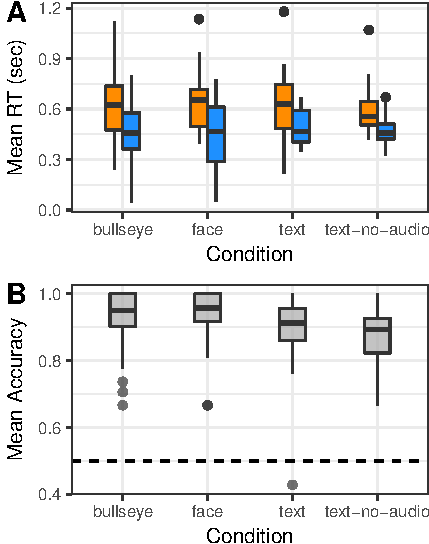
\includegraphics{figs/e2_plot-1} 

}

\caption[Behavioral and model-based results from Experiment 2 for all center stimulus types]{Behavioral and model-based results from Experiment 2 for all center stimulus types. Panel A shows reaction times, Panel B shows accuracy, and Panel C shows the output of the EWMA guessing model. All plotting conventions are the same as in Figures 2 and 3.}\label{fig:e2_plot}
\end{figure*}
\end{CodeChunk}

\section{Experiment 2}\label{experiment-2}

The goal of Experiment 2 was to replicate a key finding from Experiment
1: that increasing the competition between attention language and
attention to the visual world reduces the proportion of
nonlanguage-driven shifts. Moreover, we set out to conduct a
confirmatory test of our account that also controlled for the population
differences in Experiment 1. To accomplish these goals, we tested a
sample of English-speaking adults using a within-participants
manipulation of the center stimulus type. We used the Face and Bullseye
stimulus sets from Experiment 1\footnote{We chose not to include the
  Object stimulus set because performance between the Bullseye and
  Object tasks was indistinguishable in Experiment 1.} and added two new
conditions: Text, where the verbal language information was accompanied
by an unfolding display of printed text, and Text-no-audio, where the
spoken language stimuli were removed (see Figure 1 for an example of the
text display). The key behavioral prediction is that participants in the
Text conditions (where the center stimulus provides information about
the linguistic stimulus) should produce a higher proportion of
language-driven shifts and fewer exploratory shifts to the visual world.
We did not predict a difference in the DDM analysis since adults were
responding to highly familiar words with only two response options.

\subsection{Method}\label{method-1}

\subsubsection{Participants}\label{participants-1}

25 Stanford undergraduates participated (6 male, 20 females) for course
credit. All participants were monolingual, native English speakers and
had normal vision.

\subsubsection{Stimuli}\label{stimuli-1}

Audio and visual stimuli were identical to the Face and Bullseye tasks
in Experiment 1. We included a new center fixation stimulus type:
printed text. The text was displayed in a white font on a black
background. The text was programmed such that only a single word
appeared on the screen at a time with each word appearing for the same
duration as the corresponding word in the spoken language stimuli.

\subsubsection{Design and procedure}\label{design-and-procedure-1}

The design was nearly identical to Experiment 1, with the exception of
the change to a within-subjects manipulation where each participant
completed all four tasks (Bullseye, Face, Text, and Text-no-audio). In
both the Text and Text-no-audio conditions, the center stimulus was
white text printed on a black background. In the Text condition, spoken
language accompanied the printed text. In the Text-no-audio condition,
the spoken language stimuli was remvoed. Participants viewed each task
on a 27" monitor and were told their eye movements would be recorded.
Participants saw four blocks of 32 test trials for a total of 128
trials. Participants' eye movements were tracked using automated
eye-tracking software from SensoMotoric Instruments (SMI), sampling at
120 Hz.

\subsection{Results and Discussion}\label{results-and-discussion-1}

\subsubsection{Behavioral analyses}\label{behavioral-analyses-1}

\emph{RT.} Panel A of Figure 5 shows adults' RTs for correct and
incorrect shifts. Visual inspection of the figure suggests that there
was a speed-accuracy tradeoff in all conditions: incorrect RTs tended to
be faster than correct RTs. We fit a linear mixed-effects regression
with the same specification as in Experiment 1, but we added by-subject
intercepts and slopes for each center stimulus type to account for our
within-subjects condition manipulation. We did not find evidence that
RTs were different across conditions (all p \textgreater{} .05).

\emph{Accuracy.} Next, we compared the accuracy of first shifts across
the different tasks by fitting a mixed-effects logistic regression with
the same specifications (see Panel B of Figure 5). We found that
participants tended to be less accurate in the Text conditions compared
to conditions without text (\(\beta\) = -0.62, \(p\) \textless{} .001).
We did not find evidence for any of the other comparisons.

\subsubsection{Model-based analyses}\label{model-based-analyses-1}

\emph{EWMA} Panel C of Figure 5 shows the output of the EWMA model for
the four different center stimulus types. In contrast to Experiment 1,
we found that the CS crosses the UCL in all four conditions, suggesting
that at some point in the RT distribution adults' shifts are driven by
seeking out the named referent. Interestingly, we found a graded effect
of condition on the location when the CS crossed the UCL such that the
Text-no-audio condition occurred first (see the vertical dashed lines in
Figure 5), followed by the Text and Face conditions that were not
different from one another, and finally the Bullseye condition (TODO
stats). We also found the same graded difference in the proportion of
shifts that occurred while the CS was below the UCL, indicating a higher
proportion of first shifts were language-driven in the Text conditions
(TODO stats). These results provide strong evidence for our key
prediction: that increasing the value of fixating the center stimulus
for gathering language information reduces the probability of eye
movements to gather information about the visual world.

\emph{DDM.} Using the output of the EWMA, we fit the same hierarchical
DDM as in Experiment 1 to test if there were differences in the timing
and accuracy of responses generated by the incoming linguistic signal.
There was a high overlap of the posterior distributions for both the
boundary separation and the drift rate parameters, providing evidence
that the estimates did not differ across conditions.

Short summary of E2 results here.

\section{General Discussion}\label{general-discussion}

Language comprehension involves a tradeoff between gathering linguistic
information and gathering information about the surrounding world. In
the current work, we propose that eye movements during language
processing reflect a sensitivity to the value of gathering different
kinds of information. We found that, young ASL-learners generated slower
but more accurate shifts away from a language source andproduced a
smaller proportion of nonlanguage-driven shifts. We found the same
pattern of behavior within a sample of English-speaking adults
processing displays of printed text compared to spoken language. These
results suggest that as the value of fixating on a loaction to gathering
information about language increases, eye movements to gather
information about the visual world become less useful and occur less
frequently.

There are several limitations to our experiments. First, we have not
performed a confirmatory test of the DDM findings (ASL-learners
prioritization of accuracy over speed) from Experiment 1. So this
finding, while interesting, is preliminary. Second, we do not know what
might be driving the population differences in Experiment 1. It could be
that ASL-learners massive experience dealing with competition for visual
attention leads to changes in the deployment of eye movements during
language comprehension. Or, it could be that the in-the-moment
constraints of processing a visual language causes different fixation
behavior. Finally, we used a very simple visual world, with only three
places to look, and very simple linguistic stimuli, especially for the
adults in Experiment 2. Thus it remains an open question how these
results might scale up to more complex language information and visual
environments.

A strength of this work is the attempt to integrate top-down, goal-based
models of vision with work on language-driven eye movements. While we
chose to start with two particular case studies -- ASL and text
processing -- we think the account is more general and that there are
many real world situations where people must negotiate the tradeoff
between gathering more information about language or about the world:
e.g., processing spoken language in noisy environments or at a distance;
or early in language learning when children are acquiring new words and
often rely on nonlinguistic cues to reference such as pointing or eye
gaze. Overall, we hope this work contributes to a broader account of eye
movements during language comprehension that can explain fixation
behaviors across wider variety of populations and processing contexts.

\section{Acknowledgements}\label{acknowledgements}

We are grateful to the families who participated in this research and to
the California School for the Deaf in Fremont for their help with
participant recruitment. This work was supported by a National Science
Foundation Graduate Research Fellowship to KM and a NIDCD grant to Anne
Fernald and David Corina (DC012505).

\section{References}\label{references}

\setlength{\parindent}{-0.1in} \setlength{\leftskip}{0.125in} \noindent

\hypertarget{refs}{}
\hypertarget{ref-allopenna1998tracking}{}
Allopenna, P. D., Magnuson, J. S., \& Tanenhaus, M. K. (1998). Tracking
the time course of spoken word recognition using eye movements: Evidence
for continuous mapping models. \emph{Journal of Memory and Language},
\emph{38}(4), 419--439.

\hypertarget{ref-altmann2007real}{}
Altmann, G., \& Kamide, Y. (2007). The real-time mediation of visual
attention by language and world knowledge: Linking anticipatory (and
other) eye movements to linguistic processing. \emph{Journal of Memory
and Language}, \emph{57}(4), 502--518.

\hypertarget{ref-ballard2009modelling}{}
Ballard, D., \& Hayhoe, M. (2009). Modelling the role of task in the
control of gaze. \emph{Visual Cognition}, \emph{17}(6-7), 1185--1204.

\hypertarget{ref-bates2013lme4}{}
Bates, D., Maechler, M., Bolker, B., \& Walker, S. (2013). Lme4: Linear
mixed-effects models using eigen and s4. r package version 1.0-5.

\hypertarget{ref-hayhoe2005eye}{}
Hayhoe, M., \& Ballard, D. (2005). Eye movements in natural behavior.
\emph{Trends in Cognitive Sciences}, \emph{9}(4), 188--194.

\hypertarget{ref-ratcliff2015individual}{}
Ratcliff, R., \& Childers, R. (2015). Individual differences and fitting
methods for the two-choice diffusion model of decision making.
\emph{Decision}, \emph{2}(4), 237--279.

\hypertarget{ref-salverda2011goal}{}
Salverda, A. P., Brown, M., \& Tanenhaus, M. K. (2011). A goal-based
perspective on eye movements in visual world studies. \emph{Acta
Psychologica}, \emph{137}(2), 172--180.

\hypertarget{ref-shadlen2013decision}{}
Shadlen, M. N., \& Kiani, R. (2013). Decision making as a window on
cognition. \emph{Neuron}, \emph{80}(3), 791--806.

\hypertarget{ref-tanenhaus1995integration}{}
Tanenhaus, M. K., Spivey-Knowlton, M. J., Eberhard, K. M., \& Sedivy, J.
C. (1995). Integration of visual and linguistic information in spoken
language comprehension. \emph{Science}, \emph{268}(5217), 1632.

\hypertarget{ref-vandekerckhove2007fitting}{}
Vandekerckhove, J., \& Tuerlinckx, F. (2007). Fitting the ratcliff
diffusion model to experimental data. \emph{Psychonomic Bulletin \&
Review}, \emph{14}(6), 1011--1026.

\hypertarget{ref-wiecki2013hddm}{}
Wiecki, T. V., Sofer, I., \& Frank, M. J. (2013). HDDM: Hierarchical
bayesian estimation of the drift-diffusion model in python.
\emph{Frontiers in Neuroinformatics}, \emph{7}, 14.

\end{document}
